\AL[MS]{1.5 pages}

We now present the Snooze framework for VM
management~\cite{feller:ccgrid12} as a second case study of how
to implement and simulate advanced algorithms.

\subsubsection{Overview}

We first briefly present the Snooze architecture summarizing its main
characteristics from its presentation~\cite{feller:ccgrid12} and
additional info stemming from personal communications of the Snooze
developers and its implementation~\cite{snoozedev14,snoozeweb}.

\begin{figure}
  {\centering ~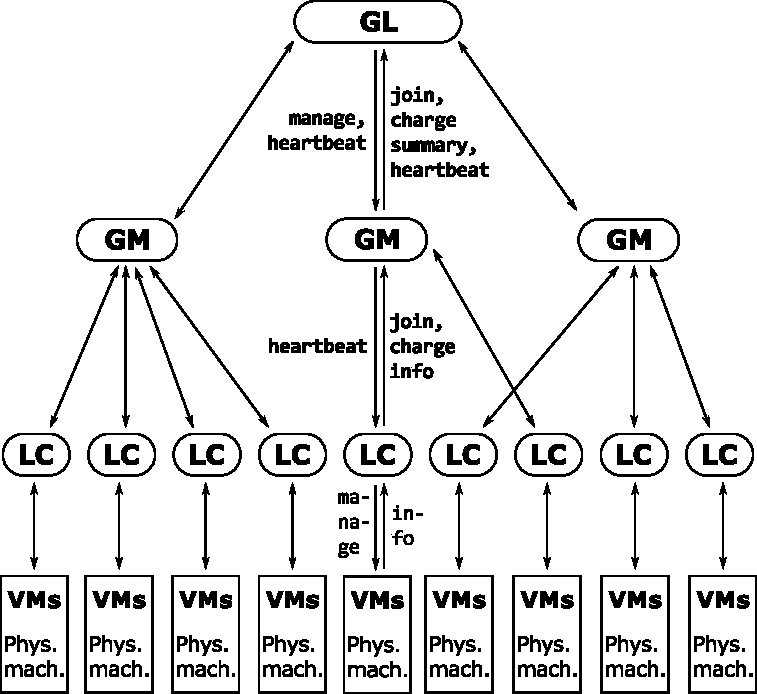
\includegraphics[width=.95\linewidth]{figures/snoozearch.pdf}}
  \caption{Overview of Snooze's architecture}
  \label{fig:snoozearch}
\end{figure}

\paragraph{Architecture}

Snooze harnesses a hierarchical architecture in order to support load
balancing and fault tolerance, see Fig.~\ref{fig:snoozearch}. At the
top of the hierarchy, a \emph{group leader (GL)} centralizes
information about the whole cluster by keeping summary information
about all \emph{group managers (GMs)} that constitute the intermediate
layer of the hierarchy. GMs manage a number of \emph{local controllers
  (LCs)}, each of which represent a node in a cluster and manage the
VMs assigned to that node. During execution, higher level components
periodically send heartbeats to lower-level components; monitoring
information, \eg on the system load, is also sent periodically in the
opposite direction. In order to propagate information down the
hierarchy, Snooze relies on hardware support for multicast
communication. Finally, a number of replicated entry points allows
clients to contact the GL, \eg in order to submit new VMs for
integration into the system.

\paragraph{Algorithms}
\label{sec:snoozeAlgs}

Apart from the handling of faults (described below), two types of
algorithms are of major importance for the administration of the
Snooze architecture: the algorithms that enable components to
dynamically enter the system and the algorithms that propagate info
between the components.

A GL is created, if it does not exist, by promotion of a GM that is
selected according to some leader election algorithm. When a GM joins
a cluster, it starts listening on a predefined channel for the
heartbeat of the GL and registers once it has received the
heartbeat. New LCs first also wait for the GL heartbeat, request a GM
assignment from the GL and register at the GM assigned to them.

Information that is passed within the system consists in periodic
heartbeat message from the GL, GMs and LCs as well as, also periodic,
charge information from LCs sent to their respective GMs and summary
charge info sent by GMs to the GL.


\paragraph{Fault tolerance}

GLs, GMs and LCs may fail during the system execution. System
components identify that a node on the corresponding higher-level node
has failed (the GL in case of a GM, a GM in the case of an LC) in an
asynchronous fashion through the lack of heartbeat messages.

In the case of a GL failure, one of the GMs becomes the new GL, stops
its GM activities and prevents the LCs it manages so that they can
start rejoining the system. If a GM fails, the GL and the LCs it has
managed will become aware of it based on the lack of heartbeats,
update its data structures and, for the LCs, rejoin the system. If an
LC fails, its GM will finally learn of it due to the missing heartbeat
and charge information of the LC. The GM will then remove the LC from
its data structures.

\subsubsection{Simulation using Simgrid}

Snooze can be simulated using our model and tool support in a direct
and natural manner. The extended abstractions \todo{Refer to
  Sec.~\ref{sec:overview}} for hosts (\texttt{XHOST}) and VMs
(\texttt{XVM}) provide low-level facilities for scheduling algorithms
that facilitate the implementation of the Snooze simulation. We have
harnessed these facilities in order to implement core characteristics
of Snooze: the monitoring of all VMs that are part of an LC and the
migration of all VMs of the set of LCs that are managed by a GM.

The remaining concepts and algorithms of Snooze are implemented using
means of our framework, the facilities provided by Simgrid and
standard Java mechanisms. Communication between Snooze actors is
implemented based on Simgrid's primitives for, mainly asynchronous,
event handling; in particular, hardware-supported multicast
communication that is used, for example, in order to relay heartbeats
is implemented as a dedicated actor that manages a state representing
GL and GM heartbeat groups and relaying heartbeat events.

The Snooze simulation uses, as its original counterpart, a
multi-threaded implementation in order to optimize reactivity even for
large groups of LCs (or GMs) that have to be managed by one GM (or
GL).

\subsubsection{Variants}

Our simulation framework facilitates the simulation of variants of the
basic Snooze model. In the following, we present three non-trivial
evolutions that we have implemented and explored: periodic vs.\
reactive scheduling, variants of the algorithms of how GMs and LCs
join the system and load balancing on the GM level.

\paragraph{Periodic vs.\ reactive scheduling}

Snooze~\cite{feller:ccgrid12} schedules VMs in a periodic fashion:
after a fixed time period a GM calls the scheduler in order to resolve
resource conflicts among the LCs it manages. The information whether a
resource conflict has to be handled is taken based on the summary
information that is periodically sent by the LCs to the GM.

We have provided an alternative, reactive, strategy to scheduling: as
soon as they occur, LCs avert their GMs of resource conflicts; the GMs
then initiate scheduling. Implementing this reactive scheme can be
done using our framework in two manners: either by implementing
additional asynchronous transmissions as a real implementation of the
necessary state updates would proceed or, in a much more lightweight
manner, through direct accesses by the GMs to the states of their
respective LCs. While the latter does not mimic a real implementation
closely, it can be harnessed to yield a valid simulation: delays
induced by communication in the ``real'' implementation, for instance,
can be easily added as part of the lightweight simulation. We have
implemented this lightweight variant of reactive scheduling.


\paragraph{Variants of the join algorithms}

The join algorithms, see Sec.~\ref{sec:snoozeAlgs}, are crucial to the
correctness of Snooze for two main reasons: (i) they have to be
efficient because they can easily form a bottleneck if large numbers
of LCs (GMs) have to be registered at a GM (LC); (ii) they are
multi-phase protocols whose correctness especially in the presence of
faults is difficult to ensure.

In order to investigate the corresponding trade-offs, we have used our
framework to implement join algorithms that may be interrupted at any
time, repeat the the on-going phase a number of times before
reinitiating, if necessary, the entire protocol. Furthermore, the join
protocol is parameterized, \eg, in the number of threads used to
handle registration requests.

Finally, our framework has enabled us to test another aspect of
Snooze's join algorithm as presented by
Feller~\etal.~\cite{feller:ccgrid12}, a strategy we call the GM rejoin
strategy (GRJ): all GMs should rejoin if a new GM enters the
system. While GRJ supports a form of load balancing (because all LCs
are reassigned to the new set of GMs), our simulation has shown that
this strategy significantly increases the time necessary for
registering GMs and LCs compared to a simpler strategy that does not
modify existing GMs in case a new GM enters the system. This handicap
is particularly pronounced if joins of GMs may be interrupted due to
faults. Concretely, experiments involving 20 GMs and 200 LCs have
shown that this strategy often multiplies the time necessary to join
all 220 components by 10 or more compared to the simple join
strategy. While the qualitative result that the more complex strategy
presented in the paper results in a more time-consuming join process
is not very surprising, the extent of the resulting degradation was
surprising.


\paragraph{Load balancing at the GM level}

LCs are assigned to GMs by the GL as part of the LC join protocol. In
Snooze's native implementation LCs are assigned in a round-robin
fashion to the known GMs. If GMs join (and leave) the system at the
same time as LCs, a round-robin strategy at join time, however, does
not ensure an even distribution. In order to evaluate the imbalance
resulting from a round-robin strategy (as well as others) we have
implemented the LC assignment protocol in a modular fashion and
applied it in diverse highly-dynamic settings in which GMs and LCs
enter the system at the same time, fail and rejoin regularly (albeit
with varying frequency). These experiments have been mostly performed
with systems involving 20 GMs and 200 LCs. They have revealed
occurrences of large imbalances that often range from 0-20 LCs per GM
and sometimes result in individual GMs totaling more then 50 LCs.

A global strategy (such as the GRJ introduced in the discussion of
join algorithms above) may ensure a quite even distribution, but at a
higher cost (possibly, a very high cost as we have shown for the GRJ).




%%% Local Variables:
%%% mode: latex
%%% TeX-master: "main"
%%% End:
